% !TeX encoding = UTF-8
\documentclass[aspectratio=169]{beamer}
\useoutertheme[progressbar=frametitle]{metropolis}
\useinnertheme{metropolis}
\definecolor{nabgray}{rgb}{0.6,0.59,0.61}
\usecolortheme[named=nabgray]{structure}

\usepackage{tikz}
\usepackage[utf8]{inputenc}
\usepackage[spanish]{babel}
\usepackage{fontspec}
\setmonofont{JetBrains Mono}
\setmainfont{Roboto}
\setsansfont{Roboto}

\usepackage{smartdiagram}
\usepackage{qtree}
\usepackage{verbatim}
\usepackage{svg}
\usepackage{graphicx}
\usepackage{color}

\definecolor{lightgray}{rgb}{0.95, 0.95, 0.95}
\definecolor{darkgray}{rgb}{0.4, 0.4, 0.4}
%\definecolor{purple}{rgb}{0.65, 0.12, 0.82}
\definecolor{editorGray}{rgb}{0.95, 0.95, 0.95}
\definecolor{editorOcher}{rgb}{1, 0.5, 0} % #FF7F00 -> rgb(239, 169, 0)
\definecolor{editorGreen}{rgb}{0, 0.5, 0} % #007C00 -> rgb(0, 124, 0)
\definecolor{orange}{rgb}{1,0.45,0.13}
\definecolor{olive}{rgb}{0.17,0.59,0.20}
\definecolor{brown}{rgb}{0.69,0.31,0.31}
\definecolor{purple}{rgb}{0.38,0.18,0.81}
\definecolor{lightblue}{rgb}{0.1,0.57,0.7}
\definecolor{lightred}{rgb}{1,0.4,0.5}
\usepackage{upquote}
\usepackage{listings}
\lstset{language=java,
	basicstyle=\footnotesize\ttfamily,
	keywordstyle=\footnotesize\color{blue}\ttfamily,
	escapeinside={<@}{@>}
}


\usebackgroundtemplate%
{%
	
\includegraphics[width=\paperwidth]{Images/Contenido}%
}


\begin{document}


{
    \usebackgroundtemplate{
\includegraphics[width=\paperwidth]{Images/portada}}
    \begin{frame}
    \end{frame}
}



\begin{frame}{Cloud native}

\begin{alertblock}{The false assumption}
By migrating to newer cloud technologies -e.g. Serverless, BaaS, Microservices- companies will automatically achieve scale -i.e. support more users with less money - and launch new faster.
\end{alertblock}


\end{frame}



\begin{frame}{Cloud native}

\textbf{Approach} for building modern computing systems on dynamic environments such as private and public clouds.

	\begin{itemize}
		\item Reactive systems
		\item 12 cloud native factors
        \item Cloud native design patterns
        \item Domain Driven Design
		\item Microservices chassis and/or service mesh
        \item Container orchestration, serverless, BaaS
        \item Cloud
	\end{itemize}

\end{frame}


\begin{frame}{Cloud native}

	\begin{itemize}
        		\item (We want) Reactive systems
        		\item (A battle tested approach is) 12 cloud native factors
                \item (Common mistakes and solutions are described by) Cloud native design patterns
                \item (Hence we divide the system with) Domain Driven Design
        		\item (And develop the systems by using) Microservices chassis and/or service mesh
                \item (Running the workloads over) Container orchestration, serverless, BaaS
                \item (Hence the) Cloud
	\end{itemize}

The Cloud Native migration projects, are in real life Macro-Projects that should be carried out properly

\end{frame}

\begin{frame}{Cloud native}

\begin{figure}
\centering
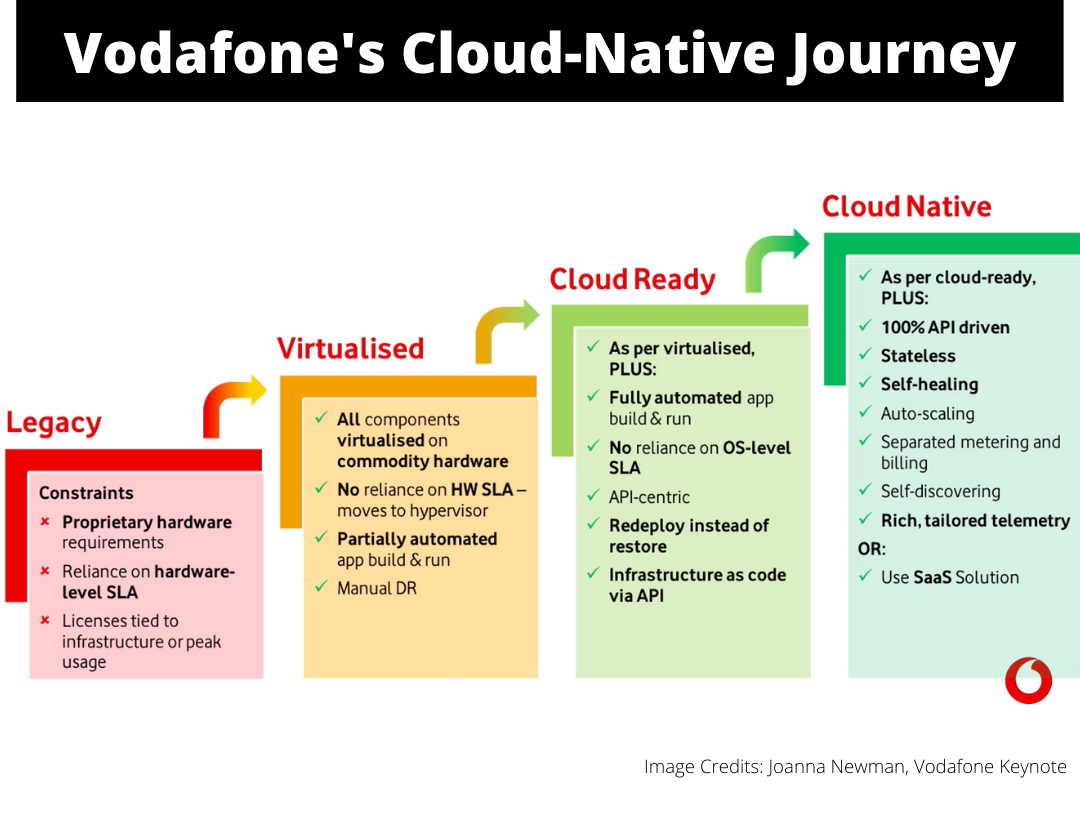
\includegraphics[width=0.6\linewidth]{Images/vodaphone}
\end{figure}
\end{frame}

{
	\usebackgroundtemplate{
\includegraphics[width=\paperwidth]{Images/separador}}
	\setbeamercolor{normal text}{fg=white}
	\setbeamercolor{frametitle}{fg=red}
	\usebeamercolor[fg]{normal text}
	\section{The migration project(s)}
}
\begin{frame}{Cloud native - The government wants to go Cloud Native}

Under NDA, but still . . .\

\begin{itemize}
 \item Government institution = Local data required by law
 \item Institution 1:
\begin{itemize}
 \item NodeJS based solution
 \item Docker based monolith
 \item CI/CD with GitLab
 \end{itemize}
  \item Institution 2:
  \begin{itemize}
   \item Java EE based solution
   \item Apache TomEE based monolith
   \item No CI/CD at all
   \end{itemize}
\end{itemize}

Both systems provide services for 16m potential users, 1000-5000 concurrent users at any time.\\


These \textbf{units} where part of the same \textbf{government sector}. 

\end{frame}

\begin{frame}{Cloud native - The PMI approach}

	\begin{itemize}
    		\item Conception \& initiation
            	\begin{itemize}
                		\item Software architecture and developer diagnose
                	\end{itemize}
    		\item Definition and planning
            	\begin{itemize}
                		\item Roadmap definition
                	\end{itemize}
            \item Launch or execution
            	\begin{itemize}
                		\item Implementation
                		\item Acquisitions 
                        \item Training
                        \item Software development
                	\end{itemize}
            \item Performance \& control
            	\begin{itemize}
                		\item Tech: Deliverable and quality metrics
                        \item Project: Budget, deadlines, viability
                	\end{itemize}
    		\item Project close
\begin{itemize}
                		\item Live documentation
                        \item Continuous improvement
                	\end{itemize}
    	\end{itemize}

\end{frame}


\begin{frame}{Conception \& initiation}
No more than two brainstorming sessions. Two hours on average\\

Mandatory stakeholders:\\
\begin{itemize}
\item Software architect (Tech Lead, Dev. Sr.)
\item Infrastructure (Sysadmin, SRE)
\item Direct contact point
\end{itemize}

Key questions:\\
\begin{itemize}
\item Motivation
\item Current team's size and skills
\item Tech Stacks
\end{itemize}
\end{frame}

\begin{frame}{Definition and planning}
Architecture review
\begin{itemize}
\item Issues
\item Possible solutions, approaches and \textbf{actions}
\item Roadmap with options (consultants, outsourcing, training)
\item Contracts based on deliverables
\end{itemize}
\end{frame}

\begin{frame}{Definition and planning}
\begin{figure}
\centering
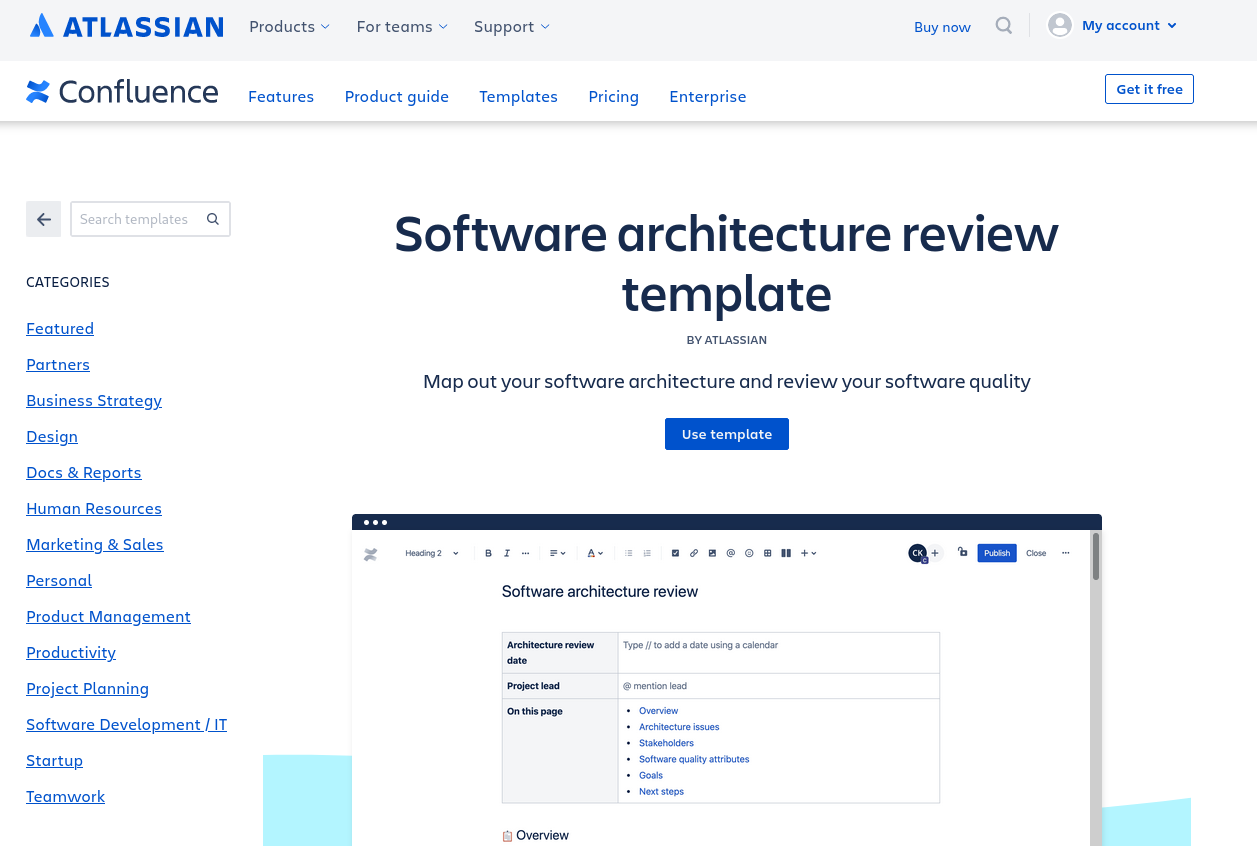
\includegraphics[width=0.7\linewidth]{Images/atlassian}
\end{figure}
\end{frame}

\begin{frame}{Definition and planning}
Project - Description - Estimated time - Provided opportunities
\begin{figure}
\centering
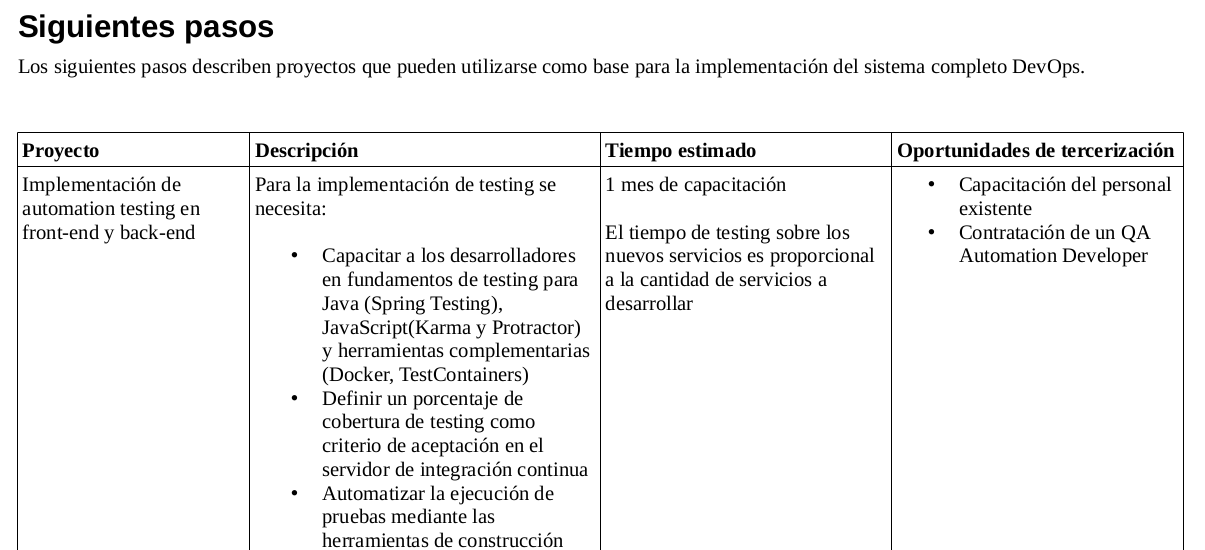
\includegraphics[width=0.8\linewidth]{Images/pasos}
\end{figure}
\end{frame}

\begin{frame}{Launch or execution}
1-Contact point, 2-Direct means of communication , 3- Non-repudiable means of communication


\begin{itemize}
    \item Culture
        \begin{itemize}
        \item DevOps
        \item Test Driven Development
        \end{itemize}
    \item  Infrastructure
        \begin{itemize}
        \item Remote access
        \item VCS, CI/CD
        \item Cloud Native Platform -e.g. Openshift, Kubernetes, Amazon EKS, Oracle Kubernetes Engine-
        \item Observability -e.g. Linkerd, Prometheus, Grafana, ELK, alarms-
        \end{itemize}
 \end{itemize}
Ideally make one presentation/technology transfer per deliverable.
\end{frame}


\begin{frame}{Launch or execution}
All phases produce \textbf{"live documentation"}.

\begin{itemize}

     \item  Training and development
        \begin{itemize}
        \item Bootstrap archetypes (also pet projects)
        \item SCM -e.g. Maven, NPM -
        \item TDD, DDD, Microservice Chassis, infrastructure as code
        \item CI/CD Pipelines
        \item Don't kill the monolith, create an ecosystems around 
        \item New project with mandatory cloud native factors
        \end{itemize}
\end{itemize}

\end{frame}


\begin{frame}{Launch or execution - DevOps}
\begin{figure}
	\centering
	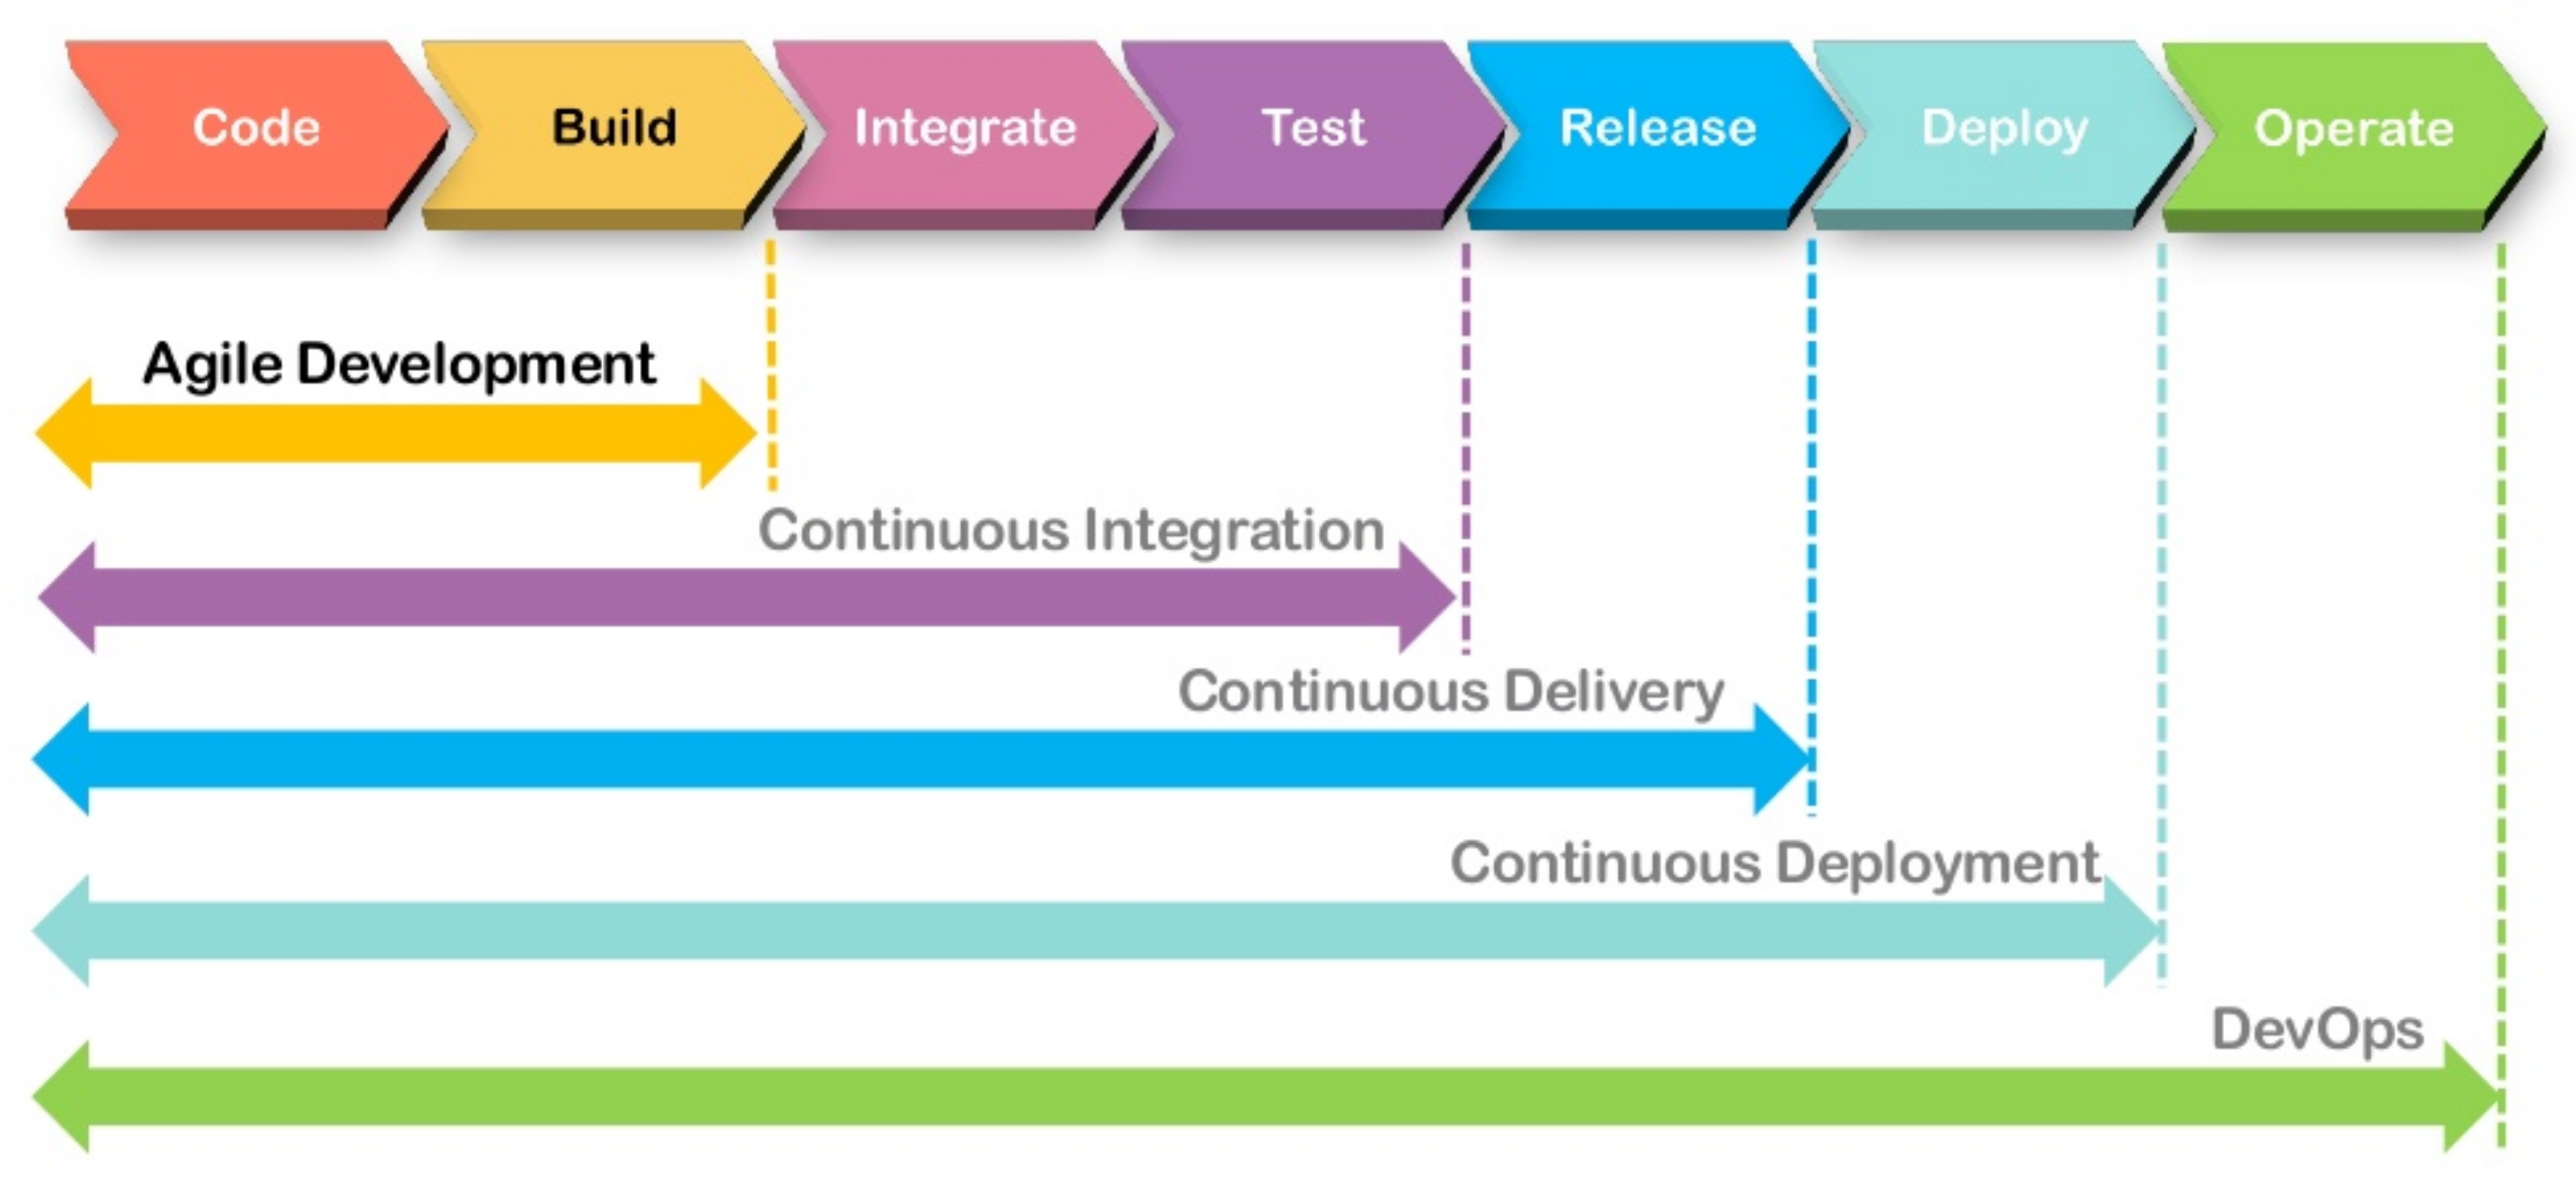
\includegraphics[width=\linewidth]{Images/etapa1}
	\label{fig:etapa1}
\end{figure}
\end{frame}

\begin{frame}{Launch or execution - CI/CD}
\begin{figure}
	\centering
	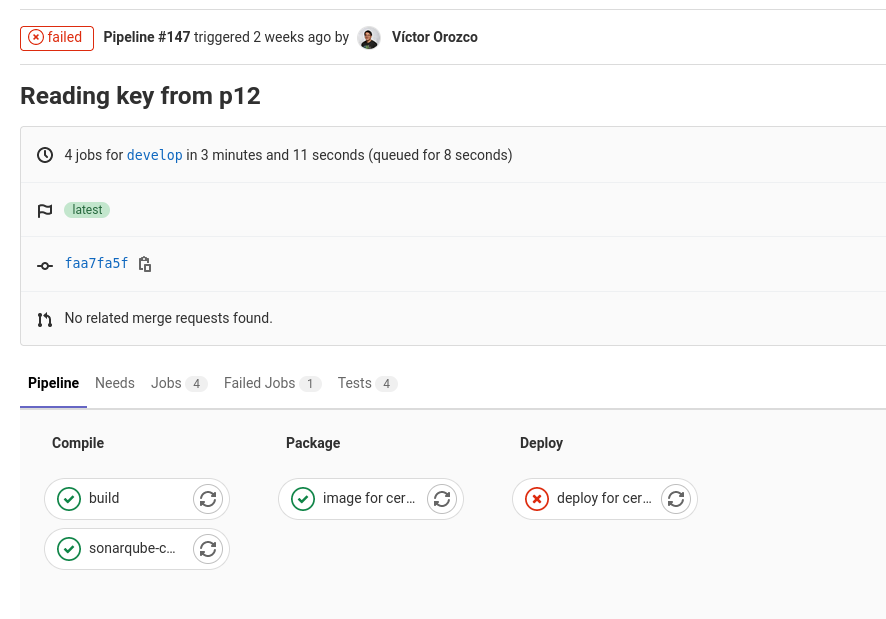
\includegraphics[width=0.7\linewidth]{Images/cicd}
\end{figure}
\end{frame}

\begin{frame}{Performance \& control}

\begin{itemize}
\item Tech
    \begin{itemize}
    \item Code quality-e.g. coverage, code smells, bugs, vulnerabilities-
    \item Performance -e.g. network latency and failures-
    \item Instrumentation
    \item How many services have been migrated 
    \end{itemize}
\item  Project
    \begin{itemize}
    \item Budget
    \item Deliverables vs. deadlines
    \item Users and developers perceptions
    \end{itemize}
\end{itemize}
\end{frame}

\begin{frame}{Performance \& control - Quality}
\begin{figure}
	\centering
	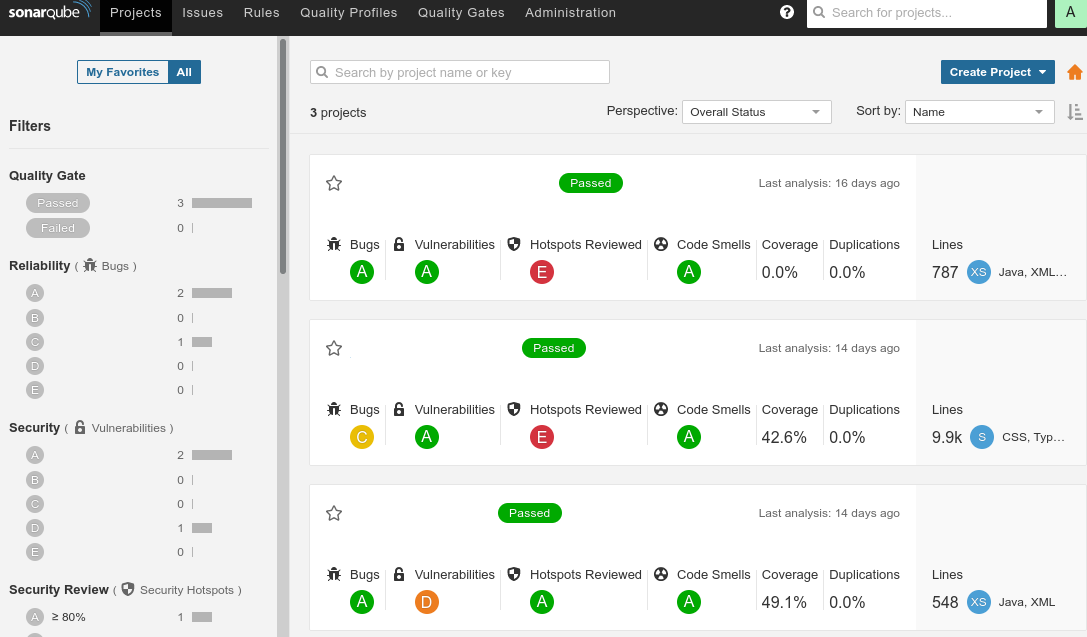
\includegraphics[width=0.8\linewidth]{Images/sonar}
\end{figure}
\end{frame}

\begin{frame}{Performance \& control - Instrumentation}
\begin{figure}
	\centering
	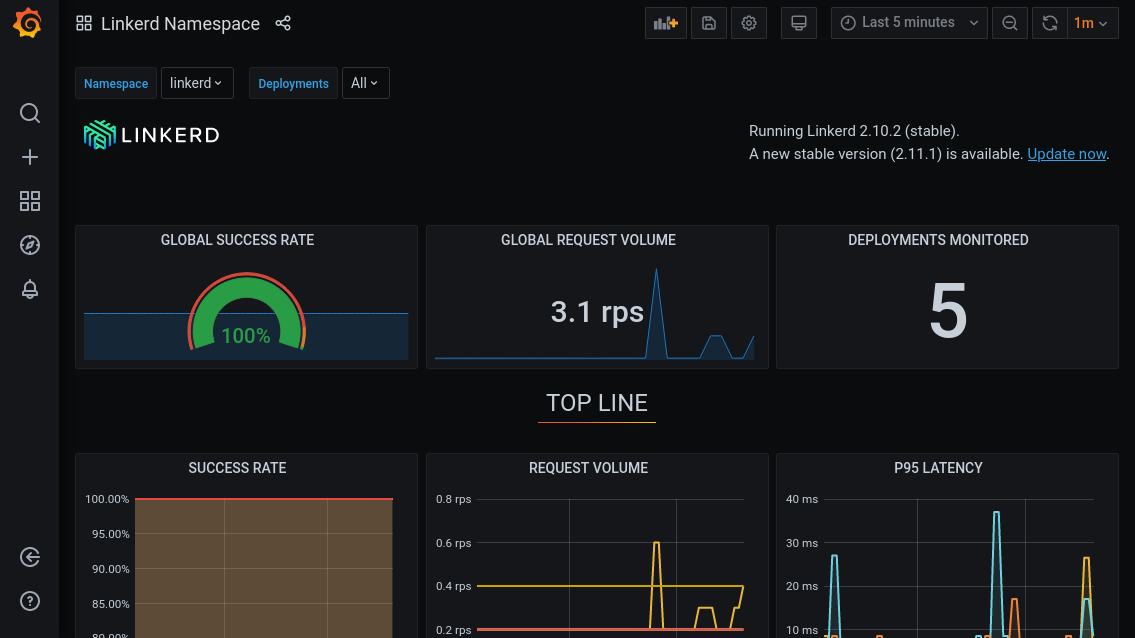
\includegraphics[width=0.8\linewidth]{Images/grafana}
\end{figure}
\end{frame}

\begin{frame}{Project close}
\begin{itemize}
\item Implementation \textbf{should} transition to support
\item Live documentation
\item What could be done better?
\end{itemize}
\end{frame}

\begin{frame}{Project close - Live documentation}
\begin{figure}
	\centering
	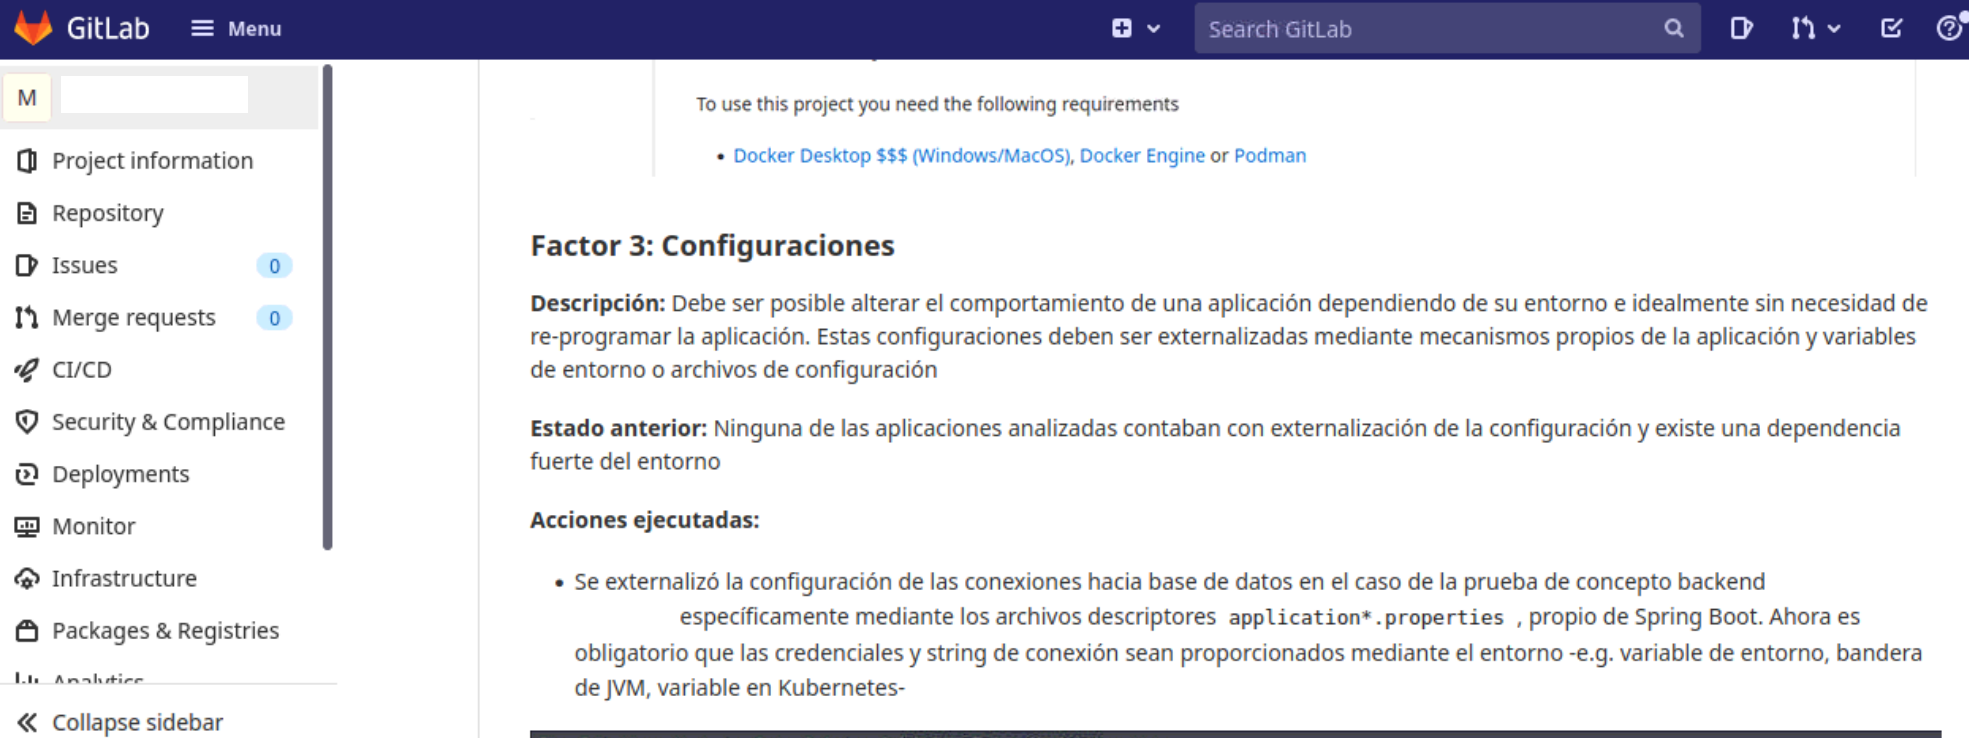
\includegraphics[width=\linewidth]{Images/docviva}
\end{figure}
\end{frame}


\begin{frame}{Víctor Orozco}
    \begin{columns}[T] % contents are top vertically aligned

        \begin{column}[T]{4cm} % alternative top-align that's better for graphics
            \begin{figure}
                \centering
                
\includegraphics[width=\linewidth]{Images/logos}
            \end{figure}
        \end{column}
        \begin{column}[T]{6cm} % each column can also be its own environment
            \begin{itemize}
                \item vorozco@nabenik.com
                \item \href{https://twitter.com/tuxtor}{@tuxtor}
                \item \href{https://vorozco.com}{https://vorozco.com}
                \item \href{https://tuxtor.shekalug.org}{https://tuxtor.shekalug.org}
            \end{itemize}
            \begin{center}
                
\includegraphics[width=0.1\linewidth]{Images/cclogo}
                \\
                This work is licensed under Creative Commons Attribution-NonCommercial-ShareAlike 3.0 Guatemala (CC BY-NC-SA 3.0 GT).
            \end{center}
        \end{column}
    \end{columns}
\end{frame}
{
    \usebackgroundtemplate{
\includegraphics[width=\paperwidth]{Images/final}}
    \begin{frame}
    \end{frame}
}


\end{document}
